\documentclass[10pt,twocolumn,letterpaper]{article}
\usepackage{graphicx}
\usepackage{amsmath}
\usepackage{amssymb}
\usepackage{booktabs}
\usepackage{nicefrac}
\usepackage{algorithm}
\usepackage[algo2e]{algorithm2e} 
\usepackage{multirow}
\usepackage[pagebackref,breaklinks,colorlinks]{hyperref}

% Support for easy cross-referencing
\usepackage[capitalize]{cleveref}
\crefname{section}{Sec.}{Secs.}
\Crefname{section}{Section}{Sections}
\Crefname{table}{Table}{Tables}
\crefname{table}{Tab.}{Tabs.}

\begin{document}
\nocite{*}

\title{Template File}
\author{The author name}
\maketitle

\section{\label{sec:Equ}Equations}

\begin{equation}
\hat{\alpha} = \arccos \left ( \sum_{i=0}^N \cos(\alpha_i)   \right)
  \label{eq:equation1}
\end{equation}

The estimation of the variable $\alpha$, called $\hat{\alpha}$, is given by the \cref{eq:equation1}.

\section{\label{sec:Fig}Figures}

\begin{figure}[H] % Tableau d'images
    \centering
    \begin{tabular}{|c|c|}
         \includegraphics[height=4cm,width=4cm]{images/fig1.png} &  
         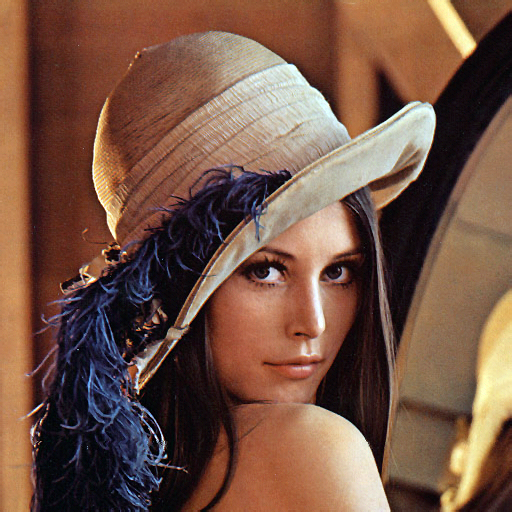
\includegraphics[height=4cm,width=4cm]{images/fig2.png} \\ 
         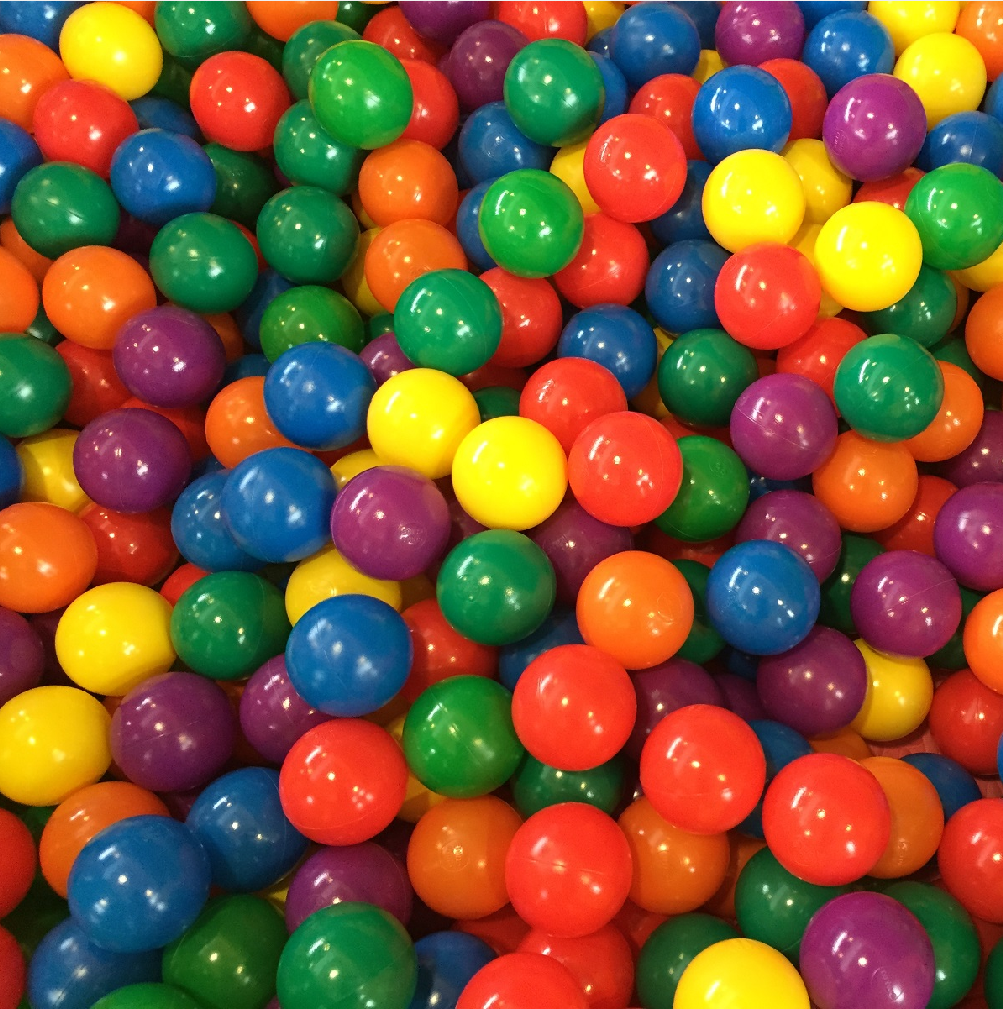
\includegraphics[height=4cm,width=4cm]{images/fig3.png} &
         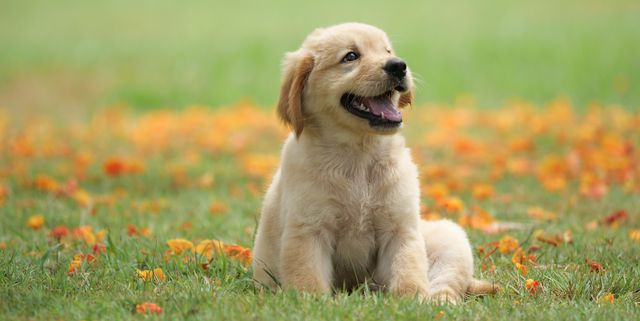
\includegraphics[height=4cm,width=4cm]{images/fig4.png} \\
    \end{tabular}
    \caption{}
    \label{fig:4figure}
\end{figure}

The images as a 2 by 2 matrix are shown in the \cref{fig:4figure}.

\section{\label{sec:Tab}Tables}

\begin{table}[H]
    \centering
    \begin{tabular}{|c|c|c|} % c : center, l : left, r : right
        \hline % trace une ligne
        Class & sub-class & quantity \\
        \hline
        \multirow{3}{5em}{Tools} & Hammer & 5 \\
        \cline{2-3}
        & Cutter & 3\\
        \cline{2-3}
        & Drill & 1\\
        \hline
    \end{tabular}
    \caption{Inventory table}
    \label{tab:inventory}
\end{table}

The inventory of the lab is detailed in \cref{tab:inventory}.

{\small
\bibliographystyle{IEEEtran}
\bibliography{references}
}

\end{document}


